A heuristic is any approach to problem solving that employs a practical method that is not fully optimized but it is sufficient to reach an immediate short-term goal or approximation.

Given the NP-Hard nature of the Travelling Salesman Problem, finding the optimal solution may require a long time, hence the need to have heuristics method to find solutions that are close to the optimal.

\section{Nearest Neighbor (Greedy)}

A first approach to the TSP is to iteratively build a solution by starting from a certain node and considering the edges with the smallest weights first when choosing the next node in the cycle.

This type of logic is called \textit{greedy}: a greedy algorithm looks for the locally optimal choice at each stage.

\begin{center}
    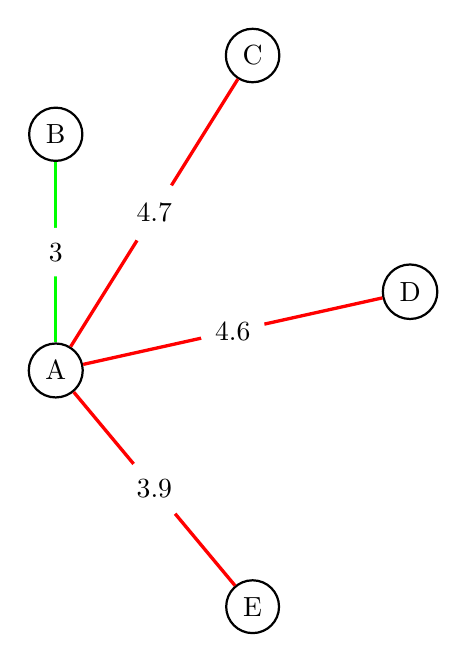
\begin{tikzpicture}
        \begin{scope}[every node/.style={circle,thick,draw}]
            \node (A) at (0,0) {A};
            \node (B) at (0,3) {B};
            \node (C) at (2.5,4) {C};
            \node (D) at (4.5,1) {D};
            \node (E) at (2.5,-3) {E};
        \end{scope}

        \begin{scope}[every node/.style={fill=white,circle},
                    every edge/.style={draw=red,very thick}]
            \path [-] (A) edge[draw=green] node {$3$} (B);
            \path [-] (A) edge node {$4.7$} (C);
            \path [-] (A) edge node {$4.6$} (D);
            \path [-] (A) edge node {$3.9$} (E);
        \end{scope}
    \end{tikzpicture}
\end{center}

In this example, among the edges connected to the node $A$, the edge $(A, B)$ is the one with the smallest weight, so node $B$ should be $A$'s successor.

By repeating this process for each new node added to the path and connecting the last node ($E$) to the starting node ($A$):

\begin{figure}[h]
    
    \centering
    \begin{subfigure}[c]{0.2\textwidth}
        \centering
        \resizebox{\linewidth}{!}{
            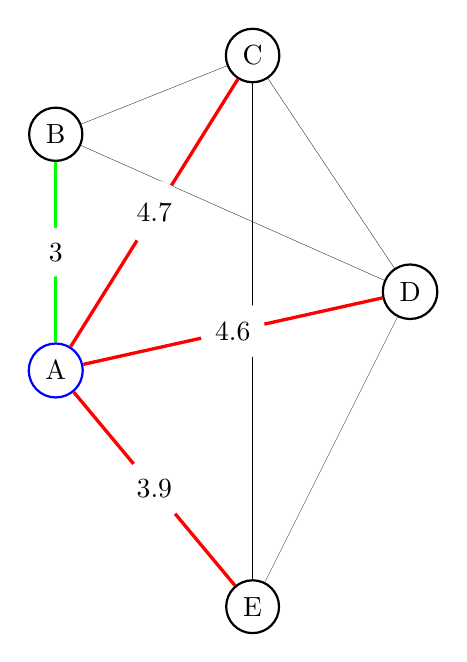
\begin{tikzpicture}
                \begin{scope}[every node/.style={circle,thick,draw}]
                    \node[draw=blue] (A) at (0,0) {A};
                    \node (B) at (0,3) {B};
                    \node (C) at (2.5,4) {C};
                    \node (D) at (4.5,1) {D};
                    \node (E) at (2.5,-3) {E};
                \end{scope}

                \begin{scope}[every node/.style={fill=white,circle},
                            every edge/.style={draw=red,very thick}]
                            \path [-] (B) edge[draw=black, ultra thin] (C);
                            \path [-] (B) edge[draw=black, ultra thin] (D);
                            \path [-] (C) edge[draw=black, ultra thin] (D);
                            \path [-] (C) edge[draw=black, ultra thin] (E);
                            \path [-] (D) edge[draw=black, ultra thin] (E);
                            \path [-] (A) edge[draw=green] node {$3$} (B);
                            \path [-] (A) edge node {$4.7$} (C);
                            \path [-] (A) edge node {$4.6$} (D);
                            \path [-] (A) edge node {$3.9$} (E);
                \end{scope}
            \end{tikzpicture}
        }
    \end{subfigure}$\Rightarrow$
    \begin{subfigure}[c]{0.2\textwidth}
        \centering
        \resizebox{\linewidth}{!}{
            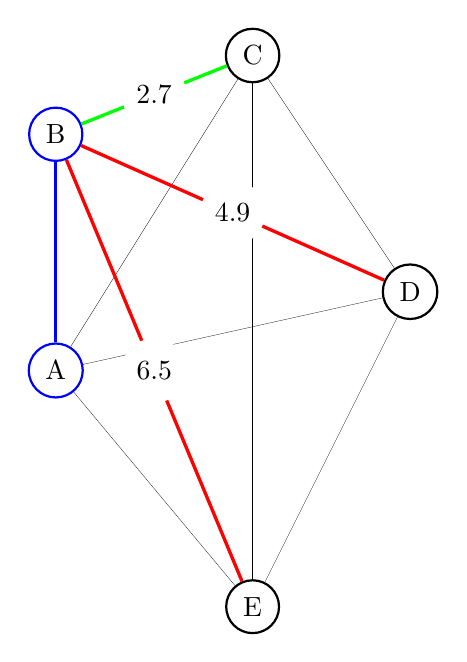
\begin{tikzpicture}
                \begin{scope}[every node/.style={circle,thick,draw}]
                    \node[draw=blue] (A) at (0,0) {A};
                    \node[draw=blue] (B) at (0,3) {B};
                    \node (C) at (2.5,4) {C};
                    \node (D) at (4.5,1) {D};
                    \node (E) at (2.5,-3) {E};
                \end{scope}

                \begin{scope}[every node/.style={fill=white,circle},
                            every edge/.style={draw=red,very thick}]
                    \path [-] (A) edge[draw=blue] (B);
                    \path [-] (C) edge[draw=black, ultra thin] (D);
                    \path [-] (D) edge[draw=black, ultra thin] (E);
                    \path [-] (E) edge[draw=black, ultra thin] (A);
                    \path [-] (A) edge[draw=black, ultra thin] (C);
                    \path [-] (A) edge[draw=black, ultra thin] (D);
                    \path [-] (C) edge[draw=black, ultra thin] (E);
                    \path [-] (B) edge[draw=green] node {$2.7$} (C);
                    \path [-] (B) edge[draw=red] node {$4.9$} (D);
                    \path [-] (B) edge[draw=red] node {$6.5$} (E);
                \end{scope}
            \end{tikzpicture}
        }
    \end{subfigure}$\Rightarrow$
    \begin{subfigure}[c]{0.2\textwidth}
        \centering
        \resizebox{\linewidth}{!}{
            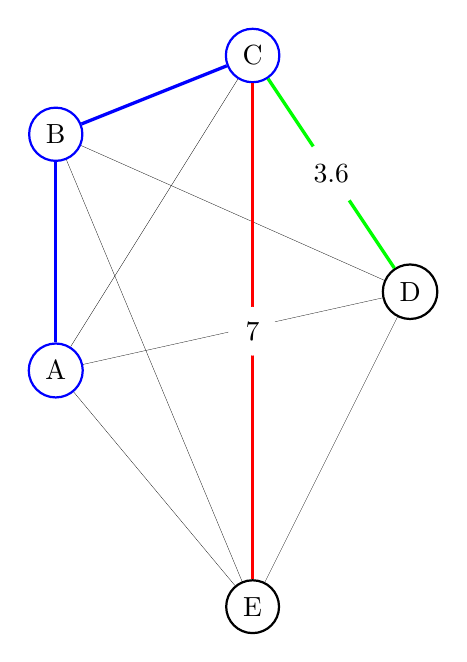
\begin{tikzpicture}
                \begin{scope}[every node/.style={circle,thick,draw}]
                    \node[draw=blue] (A) at (0,0) {A};
                    \node[draw=blue] (B) at (0,3) {B};
                    \node[draw=blue] (C) at (2.5,4) {C};
                    \node (D) at (4.5,1) {D};
                    \node (E) at (2.5,-3) {E};
                \end{scope}

                \begin{scope}[every node/.style={fill=white,circle},
                            every edge/.style={draw=red,very thick}]
                    \path [-] (A) edge[draw=blue] (B);
                    \path [-] (B) edge[draw=blue] (C);
                    \path [-] (C) edge[draw=green] node {$3.6$} (D);
                    \path [-] (D) edge[draw=black, ultra thin] (E);
                    \path [-] (E) edge[draw=black, ultra thin] (A);
                    \path [-] (A) edge[draw=black, ultra thin] (C);
                    \path [-] (A) edge[draw=black, ultra thin] (D);
                    \path [-] (B) edge[draw=black, ultra thin] (D);
                    \path [-] (B) edge[draw=black, ultra thin] (E);
                    \path [-] (C) edge[draw=red] node {$7$} (E);
                \end{scope}
            \end{tikzpicture}
        }
    \end{subfigure}$\Rightarrow$
    
\end{figure}
\begin{figure}[h]

    \centering$\Rightarrow$
    \begin{subfigure}[c]{0.2\textwidth}
        \centering
        \resizebox{\linewidth}{!}{
            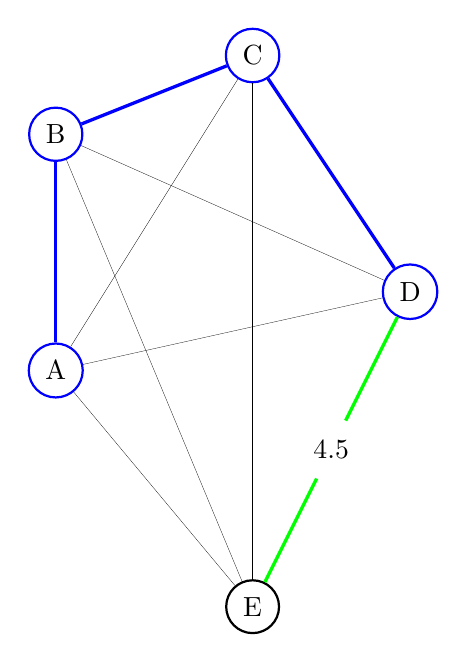
\begin{tikzpicture}
                \begin{scope}[every node/.style={circle,thick,draw}]
                    \node[draw=blue] (A) at (0,0) {A};
                    \node[draw=blue] (B) at (0,3) {B};
                    \node[draw=blue] (C) at (2.5,4) {C};
                    \node[draw=blue] (D) at (4.5,1) {D};
                    \node (E) at (2.5,-3) {E};
                \end{scope}

                \begin{scope}[every node/.style={fill=white,circle},
                            every edge/.style={draw=red,very thick}]
                    \path [-] (A) edge[draw=blue] (B);
                    \path [-] (B) edge[draw=blue] (C);
                    \path [-] (C) edge[draw=blue] (D);
                    \path [-] (E) edge[draw=black, ultra thin] (A);
                    \path [-] (A) edge[draw=black, ultra thin] (C);
                    \path [-] (A) edge[draw=black, ultra thin] (D);
                    \path [-] (B) edge[draw=black, ultra thin] (D);
                    \path [-] (B) edge[draw=black, ultra thin] (E);
                    \path [-] (C) edge[draw=black, ultra thin] (E);
                    \path [-] (D) edge[draw=green] node {$4.5$} (E);
                \end{scope}
            \end{tikzpicture}
        }
    \end{subfigure}$\Rightarrow$
    \begin{subfigure}[c]{0.2\textwidth}
        \centering
        \resizebox{\linewidth}{!}{
            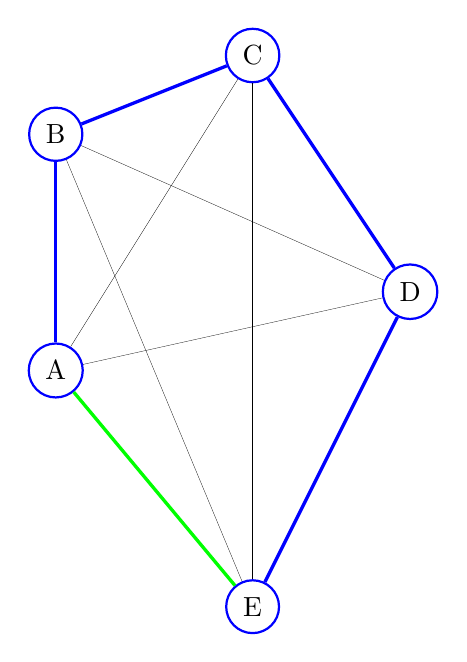
\begin{tikzpicture}
                \begin{scope}[every node/.style={circle,thick,draw}]
                    \node[draw=blue] (A) at (0,0) {A};
                    \node[draw=blue] (B) at (0,3) {B};
                    \node[draw=blue] (C) at (2.5,4) {C};
                    \node[draw=blue] (D) at (4.5,1) {D};
                    \node[draw=blue] (E) at (2.5,-3) {E};
                \end{scope}

                \begin{scope}[every node/.style={fill=white,circle},
                            every edge/.style={draw=red,very thick}]
                    \path [-] (A) edge[draw=blue] (B);
                    \path [-] (B) edge[draw=blue] (C);
                    \path [-] (C) edge[draw=blue] (D);
                    \path [-] (D) edge[draw=blue] (E);
                    \path [-] (E) edge[draw=green] (A);
                    \path [-] (A) edge[draw=black, ultra thin] (C);
                    \path [-] (A) edge[draw=black, ultra thin] (D);
                    \path [-] (B) edge[draw=black, ultra thin] (D);
                    \path [-] (B) edge[draw=black, ultra thin] (E);
                    \path [-] (C) edge[draw=black, ultra thin] (E);
                \end{scope}
            \end{tikzpicture}
        }
    \end{subfigure}$\Rightarrow$
    \begin{subfigure}[c]{0.2\textwidth}
        \centering
        \resizebox{\linewidth}{!}{
            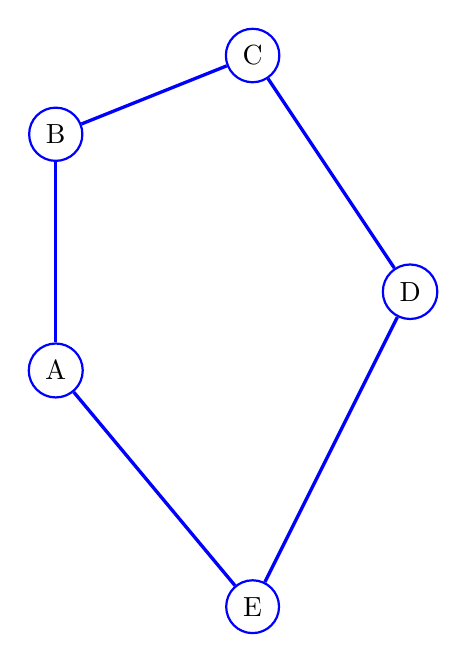
\begin{tikzpicture}
                \begin{scope}[every node/.style={circle,thick,draw}]
                    \node[draw=blue] (A) at (0,0) {A};
                    \node[draw=blue] (B) at (0,3) {B};
                    \node[draw=blue] (C) at (2.5,4) {C};
                    \node[draw=blue] (D) at (4.5,1) {D};
                    \node[draw=blue] (E) at (2.5,-3) {E};
                \end{scope}

                \begin{scope}[every node/.style={fill=white,circle},
                            every edge/.style={draw=red,very thick}]
                    \path [-] (A) edge[draw=blue] (B);
                    \path [-] (B) edge[draw=blue] (C);
                    \path [-] (C) edge[draw=blue] (D);
                    \path [-] (D) edge[draw=blue] (E);
                    \path [-] (E) edge[draw=blue] (A);
                \end{scope}
            \end{tikzpicture}
        }
    \end{subfigure}
    
\end{figure}

\FloatBarrier
\subsection{Pseudocode}
\begin{algorithm}[h]
    \caption{TSP greedy algorithm}

    \textbf{Input} starting node $s\in V$\\
    \textbf{Output} Hamiltonian cycle of V, cost of cycle\\
    \begin{algorithmic}

        \State $\mbox{cycle} \gets [s]$
        \State $\mbox{cost} \gets 0$
        
        \For{$i=0 \mbox{ to } n-2$}
            \State $\mbox{next}\gets\mbox{argmin}_v\{c(\mbox{cycle}[i],v) : v\in V - \mbox{cycle}\}$
            \State $\mbox{cost}\gets\mbox{cost}+c(cycle[i], next)$
            \State $\mbox{cycle}[i+1]\gets\mbox{next}$
        \EndFor
        \State $\mbox{cost}\gets\mbox{cost}+c(cycle[n-1],s)$\\\\
        \Return cycle, cost
    \end{algorithmic}
\end{algorithm}
\FloatBarrier

The solution found using the greedy algorithm is dependent on the starting node: a possible solution to this is to iterate through all possible starting nodes and keeping track of the best solution found so far.

\newpage

\subsection{Results analysis}
\begin{figure}[h]
    \centering
    \includegraphics*[width=.6\textwidth]{../solutions/1_600_greedy.jpg}
\end{figure}

The solutions found with the greedy algorithm are a good starting point, but sometimes the algorithm picks edges that cross a long distance, increasing the cost of the solution considerably.

This is caused by the fact that the greedy algorithm optimizes locally, without knowing whether that local choice is good or not in the long term: it might happen that after adding some edges to the cycle, the closest nodes are all already in the cycle, so the edge that will be considered may have a very large weight.

In the next section a tecnique to will fix this problem will explored.

\section{2-opt}

The 2-opt algorithm takes an existing cycle and tries to improve its cost by changing some of the edges that compose the cycle without breaking it.

The main idea behind the 2-opt algorithm is to find two edges that cross each other and fix them by removing the intersection:

\begin{figure}[h]

    \centering
    \begin{subfigure}[c]{.4\textwidth}
        \centering
        \resizebox{\linewidth}{!}{
            \begin{tikzpicture}
                \begin{scope}[every node/.style={circle,thick,draw}]
                    \node (I) at (0,0) {$p_i$};
                    \node (JJ) at (0,3) {$p_{j+1}$};
                    \node (II) at (2.5,4) {$p_{i+1}$};
                    \node (J) at (4.5,1) {$p_j$};
                \end{scope}

                \begin{scope}[>={Stealth[black]}, every node/.style={fill=white,circle},
                            every edge/.style={draw=red,very thick}]
                    \path[->] (I) edge[draw=black] (II);
                    \path[->] (J) edge[draw=black] (JJ);
                    \path[->] (JJ) edge[dashed, draw=black, thin, bend right=90] (I);
                    \path[->] (II) edge[dashed, draw=black, thin, bend left=90] (J);
                \end{scope}
            \end{tikzpicture}
        }
    \end{subfigure}
    \raisebox{-0.5\height}{$\Rightarrow$}
    \begin{subfigure}[c]{.4\textwidth}
        \centering
        \resizebox{\linewidth}{!}{
            \begin{tikzpicture}
                \begin{scope}[every node/.style={circle,thick,draw}]
                    \node (I) at (0,0) {$p_i$};
                    \node (JJ) at (0,3) {$p_{j+1}$};
                    \node (II) at (2.5,4) {$p_{i+1}$};
                    \node (J) at (4.5,1) {$p_j$};
                \end{scope}

                \begin{scope}[>={Stealth[black]}, every node/.style={fill=white,circle},
                            every edge/.style={draw=red,very thick}]
                    \path[->] (I) edge[draw=blue] (J);
                    \path[->] (II) edge[draw=blue] (JJ);
                    %\path[-] (I) edge[dashed, draw=red, thin] (II);
                    %\path[-] (J) edge[dashed, draw=red, thin] (JJ);
                    \path[->] (JJ) edge[dashed, draw=black, thin, bend right=90] (I);
                    \path[->] (J) edge[dashed, draw=blue, bend right=90] (II);
                \end{scope}
            \end{tikzpicture}
        }
    \end{subfigure}
    \caption*{$p_i\coloneq\mbox{cycle}[i]$}

\end{figure}

This process is then repeated until no more edges that can lead to an improvement to the cost of the cycle can be found.

To find a pair of edges that can be changed to improve the cost it is sufficient to find a pair of nodes $p_i$, $p_j$ that satisfies the following inequality:

$$c_{p_i,p_{i+1}}+c_{p_j,p_{j+1}} > c_{p_i,p_{j}}+c_{p_{i+1},p_{j+1}}$$

Note that the cycle list is to be considered as a circular array: situations with indexes out of bounds or $i>j$ will not be treated in this paper since the fix is trivial.

If this inequality holds then swapping the edges $(p_i,p_j),\,(p_{i+1},p_{j+1})$ with $(p_i,p_{i+1}),$ $(p_{j},p_{j+1})$ will lower the cost of the cycle:

\begin{align*}
    \mbox{cost(new cycle)}&=\mbox{cost(old cycle)}-(c_{p_i,p_{i+1}}+c_{p_j,p_{j+1}})+(c_{p_i,p_{j}}+c_{p_{i+1},p_{j+1}})\\
    &\leq\mbox{cost(old cycle)}
\end{align*}

After finding the nodes $p_i$, $p_j$ the edges $(p_i, p_j)$ and $(p_{j+1}, p_{j+1})$ will take the place of the edges $(p_i, p_{i+1})$ and $(p_j, p_{j+1})$, reversing the route connecting $p_{i+1}$ to $p_{j}$.

Suppose the cycle is stored as a list of nodes ordered following the order of the nodes in the cycle, then this step can be done simply by reversing the list from the index $i+1$ to the index $j$:

$$[\ldots,p_i,\underline{p_{i+1},\ldots,p_j},p_{j+1},\ldots]\Rightarrow[\ldots,p_i,\underline{p_j,\ldots(\mbox{reversed})\ldots,p_{i+1}},p_{j+1},\ldots]$$

\subsection{Pseudocode}
\begin{algorithm}
    \caption{TSP 2-opt algorithm}

    \textbf{Input} Hamiltonian cycle of V, cost of cycle\\
    \textbf{Output} Hamiltonian cycle of V, cost of cycle\\
    \begin{algorithmic}

        \While{*a swap improving the cost exists*}
            \State $(i, j)\gets$ *find viable swap in the cycle*
            \State $\mbox{cost}\gets\mbox{cost}-(c(p_i,p_{i+1})+c(p_j,p_{j+1}))+(c(p_i,p_{j})+c(p_{i+1},p_{j+1}))$
            \State *reverse section of cycle between indices $i+1$ and $j$*
        \EndWhile\\\\

        \Return cycle, cost

    \end{algorithmic}
\end{algorithm}

\subsection{Swap policy}

In this paper two different ways of finding a swap have been compared:

\begin{enumerate}
    \item[-] returning the first swap found that improves the cost (referred as g2opt fs)
    \item[-] looking among all possible pair of edges and returning the swap that yields the largest cost improvement (the best swap, referred as g2opt bs)
\end{enumerate}

Using the performance profiler it is easy to see that the best swap policy finds solutions with an improvement of a 1\% factor with respect to the first swap policy:

\begin{figure}[h]
    \centering
    \includegraphics*[width=.6\textwidth]{perfprof_g2opt.png}
    \caption*{20 instances, size 600, Time limit: 120s}
\end{figure}

This is due to the fact that the first swap policy might get lost in improving the solution by a small amount by finding swaps in a region with an high concentration of nodes while the best swap policy aims to improve the edges with the highest weights.

This leads the best swap policy to fix immediately the worst edges, lowering right away the cost of the solution by a large amount.

\newpage

\subsection{A faster implementation}

The 2-opt algorithm is a good asset since it improves the solutions of a factor of 15\% with respect to the greedy solution, but it requires much more time (even in the multi thread version):
\begin{figure}[h]
    \centering
    \includegraphics*[width=.6\textwidth]{perfprof_g2opt_times.png}
    \caption*{20 instances, size 600, Time limit: 120s}
\end{figure}

As we can see, the 2-opt algorithm takes 15-20 times as much to reach these improvements: this slowdown gets worse with bigger problems seen the exponential time required to solve it.\\

The time needed by the 2-opt algorithm to fix the greedy solutions depends on the number of nodes, as stated before, but also on the quality of the solution that is being improved, so if we can somehow improve the solution before using the 2-opt algorithm, the time required to complete it will be much lower.\\

The idea is then to use a Divide and Conquer approach, applying the 2-opt algorithm to 2 subproblems and then applying it to the union of the 2 solutions to the subproblems.\\

\newpage

\subsubsection{Pseudocode}
\begin{algorithm}
    \caption{TSP f2opt algorithm}

    \textbf{Input} Hamiltonian cycle of V, cost of cycle\\
    \textbf{Output} Hamiltonian cycle of V, cost of cycle\\
    \begin{algorithmic}

        \If{*reached max recursion depth*}
            \State (cycle, cost) $\gets$ *apply 2-opt to the cycle*\\
            $\quad\;\;$\Return cycle, cost
        \EndIf\\

        \While{*not reached max recursion depth*}
            \State (left, right) $\gets$ *split the cycle in two parts*
            \State (left, left\_cost) $\gets$ *apply the f2opt algorithm to the "left" part of the cycle*
            \State (right, right\_cost) $\gets$ *apply the f2opt algorithm to the "right" part of the cycle*
            \State (cycle, cost) $\gets$ *join (left, right) back into one cycle*
            \State (cycle, cost) $\gets$ *apply 2-opt to the cycle*
        \EndWhile\\\\

        \Return cycle, cost

    \end{algorithmic}
\end{algorithm}

The splitting procedure used consists in dividing the set of nodes in two parts based on their coordinates, so that in each of the two subsets obtained the nodes are close to each other.

The merging procedure consists just in gluing at random the two cycles together: trying some fancy ways of merging the two cycles would lead to a waste of computational resources since the 2-opt algorithm will be applied to the resulting cycle, probably re-arranging the edges made to glue the two cycles together.

This solution leads to a way faster algorithm thanks to having to apply the 2-opt algorithm on better solutions, bringing the slowdown down to 1.4. Another improvement that can be derived from this implementation is the fact that this version of 2-opt (called \textit{f2opt} from now on), is inherently parallel, letting us reach a slowdown of 1.2.

\begin{figure}[h]
    \centering
    \includegraphics*[width=.5\textwidth]{perfprof_f2opt_times.png}
    \caption*{20 instances, size 600, Time limit: 120s}
\end{figure}

\newpage 

\section{Comparison Greedy / 2-opt}

\begin{figure}[h]
    \centering
    \includegraphics*[width=.45\textwidth]{../plots/perfprof_heur_costs.png}
    \includegraphics*[width=.45\textwidth]{../plots/perfprof_heur_times.png}
    \caption*{20 instances, 600 nodes, time limit: 120s}
\end{figure}

The 2-opt algorithm manages to consistently improve the cost of the solutions of 15-20\% with respect to the solutions found by the greedy algorithm, while the f2opt alforithm reaches an improvement of 6-8\% whith a fraction of time needed by the basic 2-opt algorithm.

\begin{figure}[h]
    \centering
    \includegraphics*[width=.45\textwidth]{../solutions/1_600_greedy.jpg}
    \includegraphics*[width=.45\textwidth]{../solutions/1_600_g2opt.jpg}
    \caption*{20 instances, 600 nodes, time limit: 120s}
\end{figure}

As we can see, with the 2-opt algorithm, the solution is now free of crossing paths.